\documentclass[border=3pt,tikz]{standalone}

\usepackage{tikz}
\usetikzlibrary{patterns,snakes}

\begin{document}
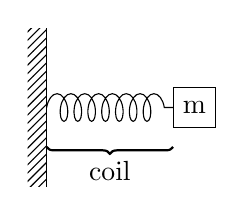
\begin{tikzpicture}
\tikzstyle{ground}=[fill,pattern=north east lines,draw=none,minimum width=0.3,minimum height=0.6]

\node (wall1) [ground, minimum height=2cm] {};
\draw (wall1.north east) -- (wall1.south east);
\node [draw,minimum width=0.5cm,minimum height=0.5cm] (mass) at (2,0) {m};
\node (fix) at (0,0) {};
\draw [
    snake=coil,
    segment amplitude=5pt,
    segment length=5pt
] (wall1.east) -- (mass); 
\draw [
    thick,
    decoration={
        brace,
        mirror,
        raise=0.5cm
    },
    decorate
] (wall1.east) -- (mass) 
node [pos=0.5,anchor=north,yshift=-0.55cm] {coil}; 
\end{tikzpicture}
\end{document}